

%In diesem Kapitel gehen wir auf die wichtigsten theoretischen Grundlagen, die für diese
%Arbeit benötigt werden, ein.

%%%%%%%%%%%%%%%%%%%%%%%%%%%%%%%%%%%%%%%%%%%%%%%%%%%%%%%%%%%%%%%%%%%%%%%%
%%%%%% Definitionen
%%%%%%%%%%%%%%%%%%%%%%%%%%%%%%%%%%%%%%%%%%%%%%%%%%%%%%%%%%%%%%%%%%%%%%%%

\section{Mathematische Definitionen}
Zu Beginn definieren wir die grundlegenden mathematischen Begriffe. Als wichtigste Grundlage dient 
hierbei das Konstrukt des ungerichteten Graphen.
\begin{definition}[Graph] ~\\
Ein (ungerichteter) \textbf{Graph} $G = (V,E)$ ist ein Tupel bestehend aus einer Knotenmenge $V$ und einer Kantenmenge
 $E$. Eine Kante verbindet zwei Knoten miteinander und ist damit eine Menge, aus zwei Knoten.
 Es gilt $E \subseteq \{ \{u,v\} |\ u,v \in V, u \neq v \}$.  
\end{definition}
\begin{definition}[Multigraph] ~\\
Ein \fett{Multigraph} $G$ ist ein Graph, in dem zwischen zwei Knoten mehrere Kanten existieren 
können. Gibt es zwischen zwei Knoten mehrere Kanten, werden diese als Multikanten bezeichnet.
\end{definition}
\noindent
In dieser Arbeit spielen bipartite Graphen, eine zentrale Rolle.
Bei einem bipartiten Graphen kann man die Knotenmenge in zwei Teilmengen teilen, sodass alle Kanten nur zwischen den 
beiden Mengen verlaufen und nicht innerhalb einer Menge. Formal bedeutet dies:
\begin{definition}[bipartiter Graph] ~\\
Ein Graph $G=(V,E)$ heißt \textbf{bipartit}, wenn es Teilmengen $V_1 \subset V$ und $V_2 \subset V$ gibt, für die 
$V_1 \cup V_2 = V$ und $V_1 \cap V_2 = \emptyset$ gilt,
 sodass für jede Kante $e \in E$ ein $u \in V_1$ und ein $v \in V_2$ existiert, sodass $e = \{u,v\}$ gilt.
Die Knotenmengen $V_1$ und $V_2$ werden auch als Partitionsklassen bezeichnet.
\end{definition}

\noindent
Ein Beispiel für einen bipartiten Graphen ist in Abbildung \ref{fig:beispiel_bipartit} dargestellt. Dabei gilt für die Partitionsklassen:
$V_1 = \{v_1,v_2,v_3\}$ und $V_2 = \{v_{4},v_5,v_6\}$. Man sieht deutlich, dass alle Kanten die Partitionenklassen
$V_1$ und $V_2$ \glqq kreuzen\grqq.

\begin{figure}
%bipartiter graph
\centering
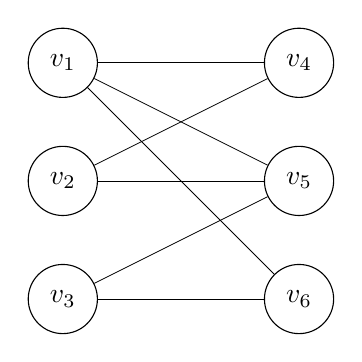
\begin{tikzpicture}
\tikzset{node style/.style={shape=circle,draw=black, inner sep=5pt,}}
                                
\node[node style] at (0, 0)     (1)     {$v_1$};
\node[node style] at (0, -1.5)   (2)     {$v_2$};
\node[node style] at (0, -3)     (3)     {$v_3$};
%\node[node style] at (0, -4.5)   (4)     {$v_4$};

\node[node style] at (3, 0)     (5)     {$v_4$};
\node[node style] at (3, -1.5)   (6)     {$v_5$};
\node[node style] at (3, -3)   (7)     {$v_6$};
%\node[node style] at (3, -4.5)   (8)     {$v_8$};

   
\draw[line width=0.1mm, >=latex]
            (1)     edge[right]    node {} (5)
            (1)     edge[right]    node {} (6)
            (1)     edge[right]    node {} (7)
            (2)     edge[right]    node {} (5)
            (2)     edge[right]    node {} (6)
            (3)     edge[right]    node {} (6)
            %(4)     edge[right]    node {} (5)
            %(4)     edge[right]    node {} (8)
            (3)     edge[right]    node {} (7)
;
\end{tikzpicture}
\caption{Beispiel eines bipartiten Graphen}
\label{fig:beispiel_bipartit}
\end{figure}
\red{überleitung
Für einen \ct{}} ist vor allem der Begriff der Nachbarschaft, genauer der gemeinsamen und disjunkten 
Nachbarschaft, entscheidend.
\begin{definition}[Nachbarschaft]~\\
Ein Knoten $u \in V$ heißt \textbf{benachbart} (oder \fett{adjazent}) zu einem 
anderen Knoten $v \in V$, wenn es eine Kante $\{u,v\} \in E $ gibt. Die Menge $N(u)$ aller adjazenten Knoten
von $u$ nennt man \fett{Nachbarschaft}.
\end{definition}
\begin{definition}[gemeinsame und disjunkte Nachbarschaft]~\\
Die \fett{gemeinsame} Nachbarschaft $N_{c}(u,v)$ zweier Knoten $u$ und $v$ ist die Menge aller Knoten, die sowohl
zu $u$ als auch zu $v$ adjazent sind. In der \fett{disjunkten} Nachbarschaft $N_{d}(u,v)$ von $u$ und $v$ sind dagegen 
alle Knoten die nur zu einem der beiden Knoten adjazent sind. \\
Es gilt also $N_{c}(u,v) = N(u) \cap N(v)$ und $N_{d}(u,v) = \big[N(u) \cup N(v)\big]\setminus \big[N(u) \cap N(v) \big]$.{}
Weiterhin gilt $N_{c}(u,v) \cap N_{d}(u,v) = \emptyset$ und $N_{c}(u,v) \cup N_{d}(u,v) = N(u) \cup N(v)$.
Jeder Knoten $x\in \left[N(u) \cup N(v)\right]$ aus den beiden Nachbarschaften liegt also entweder
in der gemeinsamen oder in der disjunkten Nachbarschaft.
\label{def:common_disjoint}
\end{definition}
\noindent
Dabei bemerken wir, dass in einem bipartiten Graphen zwei Knoten aus einer Partitionsklasse nie
in der gegenseitigen Nachbarschaft liegen können. Diesen Fakt werden wir beim Bipartiten \gc{} ausnutzen.
\blue{Zuletzt} sind noch die Begriffe Knotengrad und Gradsequenz relevant.
\begin{definition}[Knotengrad]~\\
Der \fett{Grad} eines Knotens $v \in V$ wird mit $\deg(v)$ bezeichnet und entspricht der Anzahl
der adjazenten Knoten von $v$. Es gilt also $\deg(v) = |N(v)|$ für alle Knoten $v\in V$.
\end{definition}
\begin{definition}[Gradsequenz]~\\
Die \fett{Gradsequenz} eines Graphen $G = (V,E)$ mit $|V| = n$ Knoten ist gegeben durch das Tupel
$D = (d_{1}, \dots, d_{n})$, wobei $d_{i} = \deg(v_{i})$ dem Grad des Knotens $v_{i}$ entspricht.
\end{definition}
\noindent
Im bipartiten Graph aus Abbildung \ref{fig:beispiel_bipartit} hat beispielsweise
der Knoten $v_{1}$ den Grad $\deg(v_{1}) = 3$. Für die Gradsequenz des Graphen gilt: 
$D = (3,2,2,2,3,2)$.




%%%%%%%%%%%%%%%%%%%%%%%%%%%%%%%%%%%%%%%%%%%%%%%%%%%%%%%%%%%%%%%%%%%%%%%%
%%%%%% NetworKit
%%%%%%%%%%%%%%%%%%%%%%%%%%%%%%%%%%%%%%%%%%%%%%%%%%%%%%%%%%%%%%%%%%%%%%%%
\section{\nk}

\red{\nk \cite{nk}} ist ein Open-Source Projekt, dass es zum Ziel hat, \glqq Werkzeuge für die
Analyse großer Netzwerke, in den Größenordnungen von Tausenden bis Milliarden 
von Kanten, zur Verfügung zu stellen\grqq.
\footnote{\red{aus \cite{nk}}}
\\
Innerhalb von \nk Gibt es einfache Graph Datenstrukturen \red{blabla}
\\
Man kann es mit python nutzen \red{blabla}
\blue{\Large hmmm keine Ahnung hier fehlt noch was\dots}



%%%%%%%%%%%%%%%%%%%%%%%%%%%%%%%%%%%%%%%%%%%%%%%%%%%%%%%%%%%%%%%%%%%%%%%%
%%%%%% Global Curveball
%%%%%%%%%%%%%%%%%%%%%%%%%%%%%%%%%%%%%%%%%%%%%%%%%%%%%%%%%%%%%%%%%%%%%%%%

\section{Global Curveball \red{(auf bipartiten Graphen)}}
%\red{\Huge in der bipartiten verison.....}
\label{sec:global_curveball}
\gc{} ist ein Verfahren zum Randomisieren von Graphen.
Die Aufgabe liegt also darin, bei einer gegebenen Gradsequenz $D$, eine uniform verteilte Stichprobe
aus der Menge aller Graphen mit Gradsequenz $D$ zurückzugeben. Durch das Ausführen von \gc{} 
bleibt also für jeden Knoten $v\in V$ sein Grad $\deg(v)$ erhalten. 
\\
Bei einem bipartiten \gc{} ist der Eingabegraph bipartit. Dadurch entstehen 
Vorteile, die algorithmisch ausgenutzt werden können. Zuerst behandeln wir jedoch einen einzelnen \cb{}, welcher
die Grundlage eines jeden \gc{} darstellt.
%\\
%\\
%\red{\Large
%Ein allgemeiner Ansatz wäre...
%Um dies zu erreichen kann man Kanten Tauschen....
%Was soll da dazu??}
%\\
%\\
\\
\\
\fett{\cb{}} ist  ein Prozess, bei dem Kanten zufällig getauscht werden. Bei einem \ct{} werden
zwei verschiedene Knoten $u$ und $v$ ($u\neq v$) zufällig uniform verteilt ausgewählt, deren Nachbarschaft
zufällig durchmischt wird. Da bei der bipartiten Variante  von \cb{}
die Knoten $u$ und $v$ immer beide aus der gleichen Partitionsklasse gezogen werden, ist sichergestellt, dass
es keine Kante zwischen $u$ und $v$ gibt. Somit sind die beiden Knoten nicht in der jeweils anderen Nachbarschaft
enthalten, es gilt folglich $u\notin N(v)$ und $v\notin N(u)$.
Wird die komplette Nachbarschaft \red{$N(u) \cup N(v)$ (das vielleicht einfach weglassen?)} durchmischt und wieder auf $ N(u)$ und $N(v)$ 
aufgeteilt, könnte es passieren, 
dass dadurch Multikanten entstehen,  
nämlich genau dann, wenn ein Knoten aus der gemeinsamen Nachbarschaft getauscht wird, sodass er danach in 
einer der Nachbarschaften doppelt vorkommt.
Um dies zu vermeiden werden ausschließlich die Knoten aus der disjunkten Nachbarschaft $N_{d}(u,v)$ getauscht.
Ein Beispiel für solch einen Tausch ist in Abbildung \ref{fig:curveball_trade_graph} gegeben.
%
%
%
%%%%% CURVEBALL TRADE auf graph
\begin{figure}
\centering
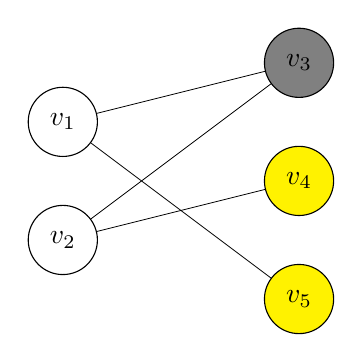
\begin{tikzpicture}
		\tikzset{node style/.style={shape=circle,draw=black, inner sep=5pt,}}
                                
\node[node style] at (0, -0.75)     (1)     {$v_1$};
\node[node style] at (0, -2.25)   (2)     {$v_2$};


\node[node style, fill=gray] at (3, 0)     (5)     {$v_3$};
\node[node style, fill=yellow] at (3, -1.5)   (6)     {$v_4$};
\node[node style, fill=yellow] at (3, -3)   (7)     {$v_5$};


   
\draw[line width=0.1mm, >=latex]
            (1)     edge[right]    node {} (5)
            (1)     edge[right]    node {} (7)
            (2)     edge[right]    node {} (5)
            (2)     edge[right]    node {} (6)

;
\end{tikzpicture}
\hspace{2cm}
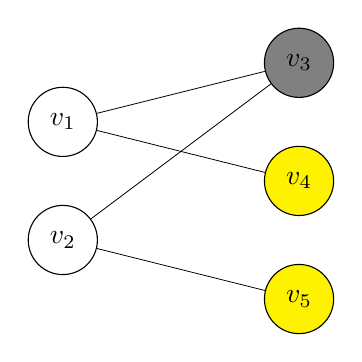
\begin{tikzpicture}
\tikzset{node style/.style={shape=circle,draw=black, inner sep=5pt,}}
                                
\node[node style] at (0, -0.75)     (1)     {$v_1$};
\node[node style] at (0, -2.25)   (2)     {$v_2$};

\node[node style, fill=gray] at (3, 0)     (5)     {$v_3$};
\node[node style, fill=yellow] at (3, -1.5)   (6)     {$v_4$};
\node[node style, fill=yellow] at (3, -3)   (7)     {$v_5$};


\draw[line width=0.1mm, >=latex]
            (1)     edge[right]    node {} (5)
            (1)     edge[right]    node {} (6)
            (2)     edge[right]    node {} (5)
            (2)     edge[right]    node {} (7)

;
\end{tikzpicture}
\caption{Es wird ein \ct{} auf den Knoten $v_{1}$ und $v_{2}$ ausgeführt. 
Für die grau markierte gemeinsame Nachbarschaft gilt $N_{c}(v_{1},v_{2}) = \{v_{3}\}$, 
die disjunkte Nachbarschaft $N_{d}(v_{1},v_{2}) = \{v_{4},v_{5}\}$ ist in gelber Farbe gekennzeichnet.
In diesem Beispiel gibt es nur die zwei gegeben Graphen, die durch Tauschen der disjunkten 
Nachbarschaft entstehen können. Ein \ct{} würde dann jeweils mit Wahrscheinlichkeit 0.5 einen der beiden 
Graphen zurückgeben.}
\label{fig:curveball_trade_graph}
\end{figure}
\\
Ein \fett{Global \ct{}} besteht aus mehreren Curveball-Tauschen, wobei möglichst jeder Knoten aus der \red{Partitionsklasse \Large auch nochmal gucken}
Teil eines Curveball-Tausches sein soll.
%
%
% 
%%%%%% Global Curveball auf partitionsarray
\begin{figure}
\centering
  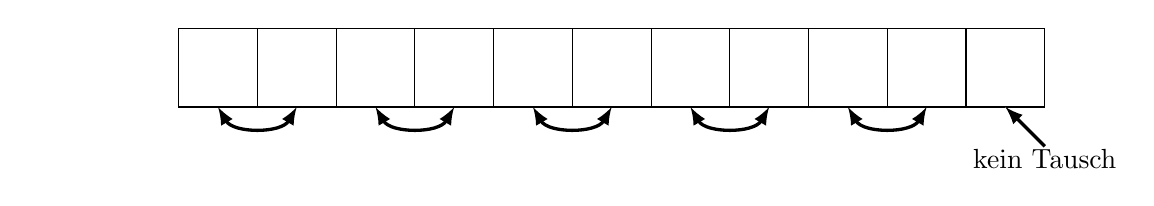
\begin{tikzpicture}[decoration=brace]
      
      
    %% COMMON FÄRBEN  
    \foreach \x in {0,1,2,3,4,5,6,7,8,9,10}
		{
			\fill [ fill =white, draw =black ]  (\x ,0) rectangle (\x+1 ,1) ;
		};
    
\node[] at (-1.8, 0.5)     (5)     {\partvek};
    
    % untere geschweifte Klammer mit Text darunter:
    \foreach \x in {0,2,4,6,8} 
 		\draw[bend angle=60,bend right,  <->,>=latex, very thick] (\x+0.5,0) to  node[below= 1ex] {\cb{}} (\x+1.5,0) ;
	
	
	\draw[bend angle=60,bend right,  <->,>=latex, very thick, color=white] (10.5,0) to  node[below= 1ex] {\textcolor{black}{kein Tausch}} (11.5,0) ;

	\draw[<-,>=latex, very thick] (10.5,0) to  node[below= 1ex] {} (11.0,-0.5) ;
%\node[] at (11.0, -0.7)     (5)     {kein Tausch};

  \end{tikzpicture}
  \caption{\gc{} auf dem zufällig permutierten \partvek}
  \label{fig:global_curveball_trade_vector}
  
\end{figure}
%
%
%
In Abbildung \ref{fig:global_curveball_trade_vector} ist eine Skizze des \partvek{s} gegeben.
Für einen \gc{} Tausch wird das Array zuerst zufällig permutiert, sodass jedes Element an einer zufälligen
Position steht.
Dann wird jeweils unabhängig ein \ct{} auf den Elementen eins und zwei, drei und vier, usw. ausgeführt.
Durch das zufällige Permutieren des Arrays zu Beginn, wird also jeder der Curveball-Tausche auf zwei zufälligen
Knoten ausgeführt. Hat das \partvek{} eine ungerade Anzahl an Elementen, bleibt am Ende ein Element übrig, 
welches nicht Teil von einem \ct{} ist. 
Hierbei können wir ausnutzen, dass der Eingabegraph bipartit ist. Da es innerhalb der Partitionsklasse \red{\Large hier nochmal gucken..}
keine zwei Knoten gibt, welche durch eine Kante miteinander verbunden sind, 
wird bei einem \ct{} auf beliebigen Knoten $u$ und $v$ 
die Nachbarschaft eines anderen Knotens $x$  aus der gleichen Partitionklasse nicht verändert. Somit
\glqq überschneiden\grqq{} sich die einzelnen Curveball-Tausche nicht. Man kann sie daher zeitgleich, 
also parallel, ausführen. Diese Parallelität führt zu einem Laufzeitvorteil.
\\
Der hauptsächliche Unterschied zwischen \gc{} auf allgemeinen und bipartiten Graphen liegt also darin, 
dass die einzelnen \ct{e} sich gegenseitig nicht beeinflussen und daher vollständig parallel behandelt werden können.
\\
\\
Im vollständigen Randomisierungs-Algorithmus werden schließlich mehrere solcher \gc{} Tausche nacheinander
durchgeführt. Die genaue Anzahl lässt sich beim Aufrufen des Algorithmus durch einen Parameter festlegen.
\\
\\
Um zu beweisen, dass das mehrfache Anwenden vom Bipartiten \gc{} eine uniform verteilte
Stichprobe aller Graphen mit gleicher Gradsequenz erzeugt, kann man das Verfahren als Markov-Kette interpretieren.
Dabei entsprechen die Zustände allen Graphen, welche eine identische Gradsequenz wie der Urspungsgraph haben.
Zwischen zwei Zuständen gibt es genau dann einen Übergang, wenn die beiden Graphen durch einen
\gc{}-Tausch ineinander überführbar sind. \red{Es lässt sich zeigen, } dass diese Markov-Kette
aperiodisch, irreduzibel und symmetrisch ist \cite{penschuck2020recent} \red{welche quelle?}. Ebenso ist die Markov-Kette endlich, da die Anzahl an
Graphen mit gegebener Gradsequenz beschränkt ist. In \cite{....?}\red{welche quelle?} wird bewiesen, dass solche
Markov-Ketten \red{zu einer uniformen Verteilung auf den Zuständen konvergiert.}





%%%%%%%%%%%%%%%%%%%%%%%%%%%%%%%%%%%%%%%%%%%%%%%%%%%%%%%%%%%%%%%%%%%%%%%%
%%%%%% Datenstruktur
%%%%%%%%%%%%%%%%%%%%%%%%%%%%%%%%%%%%%%%%%%%%%%%%%%%%%%%%%%%%%%%%%%%%%%%%

\section{Datenstruktur}
\label{sec:datenstruktur}
In \nk werden Graphen in einer eigenen Datenstruktur gespeichert.
Dabei handelt es sich um eine Art Adjazenzlistendarstellung, bei der für jeden Knoten 
in einem Array die Nachbarn gespeichert sind. Die einzelnen Knoten sind ebenfalls in
einem Array gespeichert. Da wir jedoch ausschließlich auf bipartiten ungerichteten Graphen
arbeiten, können wir eine einfachere Datenstruktur nutzen. Dazu transformieren wird den
den Graph, indem wir lediglich
die Knoten aus einer der beiden Bipartitionsklassen 
in einem Array speichern.
Welche der beiden Partitionsklassen ausgewählt wird, bleibt dem \red{Nutzer} überlassen.
Dabei ist es jedoch sinnvoll, die Klasse mit der geringeren Anzahl an Knoten zu wählen, da auf diese
Weise weniger \ct{e} auszuführen sind.
 Dieses Array werden wir als  \red{\fett{\partvek}} bezeichnen. \red{wenn im folgenden von partition gepsrochen
 wird: diese gemeint}
Für jeden dieser Knoten wird jeweils ein Array erstellt, indem alle adjazenten Knoten gespeichert sind.
Wenn $V_{1}$ die ausgewählte Partitionsklasse ist, dann gibt es also für jeden Knoten $v\in V_{1}$
ein Array, welches die Elemente aus $N(v)$ enthält.
Mit dieser Datenstruktur lassen sich effizient zwei zufällige Knoten der einen Partitionsklasse
auswählen, die (disjunkten und gemeinsamen) Nachbarschaften berechnen und Knoten aus der
disjunkten Nachbarschaft tauschen.
%
%
%
%
%
%
%%%%% CURVEBALL TRADE auf Array
\begin{figure}
\centering
  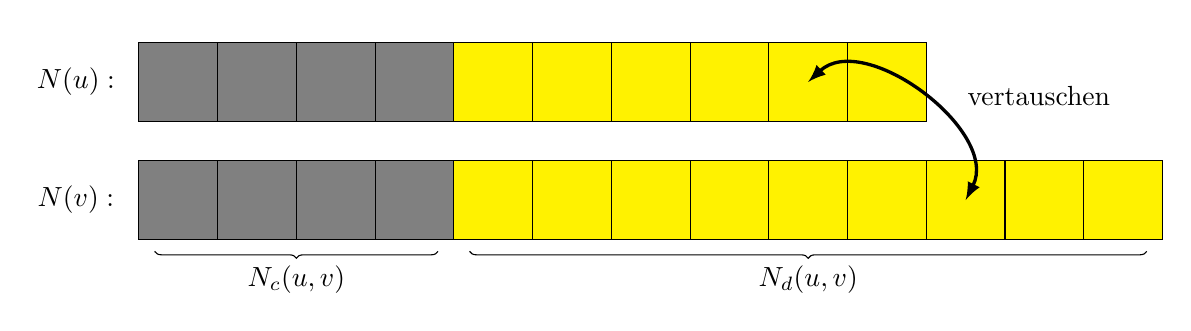
\begin{tikzpicture}[decoration=brace]
      
      
    %% COMMON FÄRBEN  
    \foreach \x in {0,1,2,3}
		{
			\fill [ fill =gray, draw =black ]  (\x ,0) rectangle (\x+1 ,1) ;
			\fill [ fill =gray, draw =black ]  (\x ,-1.5) rectangle (\x+1 ,-0.5) ;
		};

    %% DISJOINT OBEN FÄRBEN  
    \foreach \x in {4,5,6,7,8,9}
		{
			\fill [ fill =yellow, draw =black ]  (\x ,0) rectangle (\x+1 ,1) ;
		};
		
	%% DISJOINT UNTEN FÄRBEN  
    \foreach \x in {4,5,6,7,8,9,10,11,12}
		{
			\fill [ fill =yellow, draw =black ]  (\x ,-1.5) rectangle (\x+1 ,-0.5) ;
		};
    
\node[] at (-0.8, 0.5)     (5)     {$N(u):$};
\node[] at (-0.8, -1)     (5)     {$N(v):$};
    
    % untere geschweifte Klammer mit Text darunter:
    \draw[decorate, yshift=-1ex] (3.8,-1.5) -- node[below=0.4ex] {$N_{c}(u,v)$} (0.2,-1.5);
    \draw[decorate, yshift=-1ex] (12.8,-1.5) -- node[below=0.4ex] {$N_{d}(u,v)$} (4.2,-1.5);


	\draw[bend left=80, <->,>=latex, very thick] (8.5,0.5) to  node[right= 3ex] {vertauschen} (10.5,-1) ;

  \end{tikzpicture}
  \caption{Skizze eines \cb-Tausches auf den Arrays}
  \label{fig:curveball_trade_vector}
  
\end{figure}
\\
%
%
%
%
Wie ein \ct{} in der Datenstruktur, also den beiden Arrays aussieht, ist 
in Abbildung \ref{fig:curveball_trade_vector} skizziert. Dabei werden zuerst die Elemente
der beiden Vektoren in gemeinsame und disjunkte Nachbarschaft aufgeteilt. Die gemeinsame Nachbarschaft ist
wieder in grau gekennzeichnet, die disjunkte in gelb. Bei einem \ct{} bleiben dann die Elemente 
der gemeinsame Nachbarschaft unverändert, während die Elemente aus der 
disjunkten Nachbarschaft zufällig zwischen den beiden 
Arrays getauscht werden.

%%%%%%%%%%%%%%%%%%%%%%%%%%%%%%%%%%%%%%%%%%%%%%%%%%%%%%%%%%%%%%%%%%%%%%%%
%%%%%% Parallelität
%%%%%%%%%%%%%%%%%%%%%%%%%%%%%%%%%%%%%%%%%%%%%%%%%%%%%%%%%%%%%%%%%%%%%%%%

%\section{Parallelisierung}

%\red{muss hier noch was dazu?!}
